\documentclass[11pt]{article}
\usepackage{graphicx}
\usepackage{listings}
\usepackage[linesnumbered, ruled, vlined]{algorithm2e}
\usepackage{../caratuladc/caratula}
\usepackage[spanish,activeacute,es-tabla]{babel}
\usepackage[utf8]{inputenc}
\usepackage{ifthen}
\usepackage{listings}
\usepackage{dsfont}
\usepackage{subcaption}
\usepackage{amsmath}
\usepackage[strict]{changepage}
\usepackage[top=1cm,bottom=2cm,left=1cm,right=1cm]{geometry}%
\usepackage{color}%
\newcommand{\tocarEspacios}{%
	\addtolength{\leftskip}{3em}%
	\setlength{\parindent}{0em}%
}

% Especificacion de procs

\newcommand{\In}{\textsf{in }}
\newcommand{\Out}{\textsf{out }}
\newcommand{\Inout}{\textsf{inout }}

\newcommand{\encabezadoDeProc}[4]{%
	% Ponemos la palabrita problema en tt
	%  \noindent%
	{\normalfont\bfseries\ttfamily proc}%
	% Ponemos el nombre del problema
	\ %
	{\normalfont\ttfamily #2}%
	\
	% Ponemos los parametros
	(#3)%
	\ifthenelse{\equal{#4}{}}{}{%
		% Por ultimo, va el tipo del resultado
		\ : #4}
}

\newenvironment{proc}[4][res]{%
	
	% El parametro 1 (opcional) es el nombre del resultado
	% El parametro 2 es el nombre del problema
	% El parametro 3 son los parametros
	% El parametro 4 es el tipo del resultado
	% Preambulo del ambiente problema
	% Tenemos que definir los comandos requiere, asegura, modifica y aux
	\newcommand{\requiere}[2][]{%
		{\normalfont\bfseries\ttfamily requiere}%
		\ifthenelse{\equal{##1}{}}{}{\ {\normalfont\ttfamily ##1} :}\ %
		\{\ensuremath{##2}\}%
		{\normalfont\bfseries\,\par}%
	}
	\newcommand{\asegura}[2][]{%
		{\normalfont\bfseries\ttfamily asegura}%
		\ifthenelse{\equal{##1}{}}{}{\ {\normalfont\ttfamily ##1} :}\
		\{\ensuremath{##2}\}%
		{\normalfont\bfseries\,\par}%
	}
	\renewcommand{\aux}[4]{%
		{\normalfont\bfseries\ttfamily aux\ }%
		{\normalfont\ttfamily ##1}%
		\ifthenelse{\equal{##2}{}}{}{\ (##2)}\ : ##3\, = \ensuremath{##4}%
		{\normalfont\bfseries\,;\par}%
	}
	\renewcommand{\pred}[3]{%
		{\normalfont\bfseries\ttfamily pred }%
		{\normalfont\ttfamily ##1}%
		\ifthenelse{\equal{##2}{}}{}{\ (##2) }%
		\{%
		\begin{adjustwidth}{+5em}{}
			\ensuremath{##3}
		\end{adjustwidth}
		\}%
		{\normalfont\bfseries\,\par}%
	}
	
	\newcommand{\res}{#1}
	\vspace{1ex}
	\noindent
	\encabezadoDeProc{#1}{#2}{#3}{#4}
	% Abrimos la llave
	\par%
	\tocarEspacios
}
{
	% Cerramos la llave
	\vspace{1ex}
}

\newcommand{\aux}[4]{%
	{\normalfont\bfseries\ttfamily\noindent aux\ }%
	{\normalfont\ttfamily #1}%
	\ifthenelse{\equal{#2}{}}{}{\ (#2)}\ : #3\, = \ensuremath{#4}%
	{\normalfont\bfseries\,;\par}%
}

\newcommand{\pred}[3]{%
	{\normalfont\bfseries\ttfamily\noindent pred }%
	{\normalfont\ttfamily #1}%
	\ifthenelse{\equal{#2}{}}{}{\ (#2) }%
	\{%
	\begin{adjustwidth}{+2em}{}
		\ensuremath{#3}
	\end{adjustwidth}
	\}%
	{\normalfont\bfseries\,\par}%
}

% Tipos

\newcommand{\nat}{\ensuremath{\mathds{N}}}
\newcommand{\ent}{\ensuremath{\mathds{Z}}}
\newcommand{\float}{\ensuremath{\mathds{R}}}
\newcommand{\bool}{\ensuremath{\mathsf{Bool}}}
\newcommand{\cha}{\ensuremath{\mathsf{Char}}}
\newcommand{\str}{\ensuremath{\mathsf{String}}}

% Logica

\newcommand{\True}{\ensuremath{\mathrm{true}}}
\newcommand{\False}{\ensuremath{\mathrm{false}}}
\newcommand{\Then}{\ensuremath{\rightarrow}}
\newcommand{\Iff}{\ensuremath{\leftrightarrow}}
\newcommand{\implica}{\ensuremath{\longrightarrow}}
\newcommand{\IfThenElse}[3]{\ensuremath{\mathsf{if}\ #1\ \mathsf{then}\ #2\ \mathsf{else}\ #3\ \mathsf{fi}}}
\newcommand{\yLuego}{\land _L}
\newcommand{\oLuego}{\lor _L}
\newcommand{\implicaLuego}{\implica _L}

\newcommand{\cuantificador}[5]{%
	\ensuremath{(#2 #3: #4)\ (%
		\ifthenelse{\equal{#1}{unalinea}}{
			#5
		}{
			$ % exiting math mode
			\begin{adjustwidth}{+2em}{}
				$#5$%
			\end{adjustwidth}%
			$ % entering math mode
		}
		)}
}

\newcommand{\existe}[4][]{%
	\cuantificador{#1}{\exists}{#2}{#3}{#4}
}
\newcommand{\paraTodo}[4][]{%
	\cuantificador{#1}{\forall}{#2}{#3}{#4}
}

%listas

\newcommand{\TLista}[1]{\ensuremath{seq \langle #1\rangle}}
\newcommand{\lvacia}{\ensuremath{[\ ]}}
\newcommand{\lv}{\ensuremath{[\ ]}}
\newcommand{\longitud}[1]{\ensuremath{|#1|}}
\newcommand{\cons}[1]{\ensuremath{\mathsf{addFirst}}(#1)}
\newcommand{\indice}[1]{\ensuremath{\mathsf{indice}}(#1)}
\newcommand{\conc}[1]{\ensuremath{\mathsf{concat}}(#1)}
\newcommand{\cab}[1]{\ensuremath{\mathsf{head}}(#1)}
\newcommand{\cola}[1]{\ensuremath{\mathsf{tail}}(#1)}
\newcommand{\sub}[1]{\ensuremath{\mathsf{subseq}}(#1)}
\newcommand{\en}[1]{\ensuremath{\mathsf{en}}(#1)}
\newcommand{\cuenta}[2]{\mathsf{cuenta}\ensuremath{(#1, #2)}}
\newcommand{\suma}[1]{\mathsf{suma}(#1)}
\newcommand{\twodots}{\ensuremath{\mathrm{..}}}
\newcommand{\masmas}{\ensuremath{++}}
\newcommand{\matriz}[1]{\TLista{\TLista{#1}}}
\newcommand{\seqchar}{\TLista{\cha}}

\renewcommand{\lstlistingname}{Código}
\lstset{% general command to set parameter(s)
	language=Java,
	morekeywords={endif, endwhile, skip},
	basewidth={0.47em,0.40em},
	columns=fixed, fontadjust, resetmargins, xrightmargin=5pt, xleftmargin=15pt,
	flexiblecolumns=false, tabsize=4, breaklines, breakatwhitespace=false, extendedchars=true,
	numbers=left, numberstyle=\tiny, stepnumber=1, numbersep=9pt,
	frame=l, framesep=3pt,
	captionpos=b,
}

\fecha{2do cuatrimestre 2024}
\titulo{Guia 6}
\materia{Algoritmos y Estructuras de Datos}
\integrante{Prieto, Nahuel}{646/20}{enprieto@dc.uba.ar}

\graphicspath{{../static/}}

\lstset{
    morekeywords={then}                  % Define 'then' como palabra clave
}


\begin{document}
    \maketitle
    \subsection*{Ejercicio 1}
    \begin{figure}[h]
        \centering
        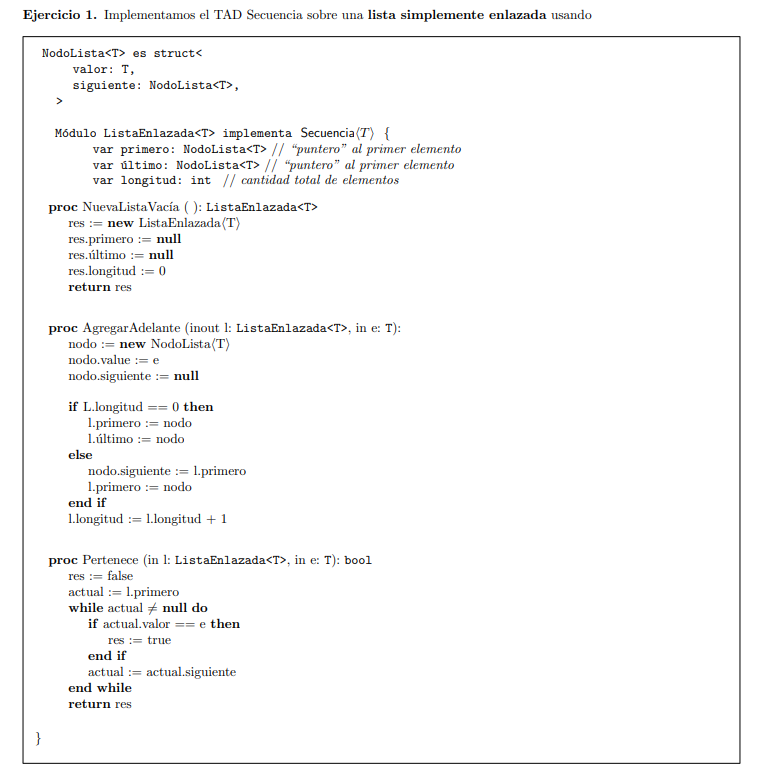
\includegraphics[width=0.9\textwidth]{../static/ejercicio1.png}
    \end{figure}
    \begin{itemize}
        \item Escriba los algoritmos para los siguientes procs y calcule su complejidad
        \begin{itemize}
            \item agregarAtras
            \item obtener
            \item eliminar
            \item concatenar
        \end{itemize}
        \item Escriba el invariante de representación para este módulo en castellano \\ \\

        \item Dado el siguiente invrep, indiquie si es correcto. En caso de no serlo, corrijalo:

        \pred{InvRep}{l: NodoLista$<$T$>$}{
            accesible(l.primero,l.ultimo) \land largoOK(l.primero,l.longitud)
        }
        \pred{largoOK}{n: NodoLista$<$T$>$, largo: \ent}{
            (n = null \land largo = 0) \lor (largoOK(n.siguiente, largo-1))
        }
        \pred{accesible}{$n_0$: NodoLista$<$T$>$, $n_1$: NodoLista$<$T$>$}{
            n_1 = n_0 \lor (n_0.siguiente \neq null \yLuego accesible(n_0.siguiente, n_1))
        }

    \end{itemize}
    \subsection*{Solucion Ejercicio 1:}
    \begin{proc}{agregarAtras}{\Inout l: ListaEnlazada$<$T$>$, \In e: T}{}
        \begin{lstlisting}
            nodo := new Nodo < T >
            nodo.valor := e
            if l.longitud = = 0 then
                l.primero := nodo
                l.ultimo := nodo
            else
                l.ultimo.siguiente := nodo
                l.ultimo := nodo
            endif
            l.longitud ++
        \end{lstlisting}
    \end{proc}

    \begin{proc}{obtener}{\In l: ListaEnlazada$<$T$>$, \In i \ent}{T}
        \begin{lstlisting}
            var actual := l.primero
            var j := 0
            while j < i do
                actual := actual.siguiente
                j++
            endwhile
            return actual.valor
        \end{lstlisting}
    \end{proc}
    \begin{proc}{eliminar}{\Inout l: ListaEnlazada$<$T$>$, \In i \ent}{}
        \begin{lstlisting}
            var eliminar := l.primero
            var j := 0
            while j < i do
                eliminar := eliminar.siguiente
                j ++
            endwhile
            if l.longitud = = 1 then
                l.primero := null
                l.ultimo = null
            else if eliminar = = l.primero
                l.primero := eliminar.siguiente
            else
                anterior := l.primero
                var k := 0
                while k < i - 1 do
                    anterior := anterior.siguiente
                    k ++
                endwhile
                if eliminar = = l.ultimo then
                    l.ultimo := anterior
                    l.ultimo.siguiente := null
                else
                    anterior.siguiente := eliminar.siguiente
                endif
                anterior := null
                anterior.siguiente = null
            endif
            eliminar.siguiente := null
            eliminar := null
        \end{lstlisting}
    \end{proc}







\end{document}